\documentclass[12pt]{article}
\usepackage[utf8]{inputenc}
\usepackage{graphicx} % Allows you to insert figures
\usepackage{amsmath} % Allows you to do equations
\usepackage{fancyhdr} % Formats the header
\usepackage{geometry} % Formats the paper size, orientation, and margins
\usepackage{caption}
\usepackage{subcaption}
\usepackage{biblatex} %Imports biblatex package
\linespread{1.25} % about 1.5 spacing in Word
\setlength{\parindent}{0pt} % no paragraph indents
\setlength{\parskip}{1em} % paragraphs separated by one line
\usepackage[style=authoryear-ibid,backend=biber,maxbibnames=99,maxcitenames=2,uniquelist=false,isbn=false,url=true,eprint=false,doi=true,giveninits=true,uniquename=init]{biblatex} % Allows you to do citations - does Harvard style and compatible with Zotero
\urlstyle{same} % makes a nicer URL and DOI font 
\AtEveryBibitem{
    \clearfield{urlyear}
    \clearfield{urlmonth}
} % removes access date
\AtEveryBibitem{\clearfield{month}} % removes months in bibliography
\AtEveryCitekey{\clearfield{month}} % removes months in citations
\renewbibmacro{in:}{} % Removes the "In" before journal names

\renewbibmacro*{editorstrg}{%from biblatex.def
  \printtext[editortype]{%
    \iffieldundef{editortype}
      {\ifboolexpr{
         test {\ifnumgreater{\value{editor}}{1}}
         or
         test {\ifandothers{editor}}
       }
         {\bibcpstring{editors}}
         {\bibcpstring{editor}}}
      {\ifbibxstring{\thefield{editortype}}
         {\ifboolexpr{
            test {\ifnumgreater{\value{editor}}{1}}
            or
            test {\ifandothers{editor}}
          }
            {\bibcpstring{\thefield{editortype}s}}%changed
            {\bibcpstring{\thefield{editortype}}}}%changed
         {\thefield{editortype}}}}}

\renewbibmacro*{byeditor+others}{%from biblatex.def
  \ifnameundef{editor}
    {}
    {\printnames[byeditor]{editor}%
     \addspace%added
     \mkbibparens{\usebibmacro{editorstrg}}%added
     \clearname{editor}%
     \newunit}%
  \usebibmacro{byeditorx}%
  \usebibmacro{bytranslator+others}}
  % The commands above from lines 20-49 change the way editors are displayed in books
\AtEveryBibitem{%
  \clearlist{language}%
} % removes language from bibliography
\citetrackerfalse 
% Removes ibids (ibidems)
\DeclareNameAlias{sortname}{family-given} % Ensures the names of the authors after the first author are in the correct order in the bibliography
\renewcommand*{\revsdnamepunct}{} % Corrects punctuation for authors with just a first initial
\addbibresource{Example.bib} % Tells LaTeX where the citations are coming from. This is imported from Zotero
\usepackage[format=plain,
            font=it]{caption} % Italicizes figure captions
\usepackage[english]{babel}
\usepackage{csquotes}
\renewcommand*{\nameyeardelim}{\addcomma\space} % Adds comma in in-text citations
\renewcommand{\headrulewidth}{0pt}
\geometry{letterpaper, portrait, margin=1in}
\setlength{\headheight}{14.49998pt}

\newcommand\titleofdoc{Credit Risk Prediction} %%%%% Put your document title in this argument
\newcommand\GroupName{Team 6} %%%%% Put your group name here. If you are the only member of the group, just put your name

\begin{document}
\begin{titlepage}
   \begin{center}
        \vspace*{4cm} % Adjust spacings to ensure the title page is generally filled with text

        \Huge{\titleofdoc} 

        \vspace{0.5cm}
        \LARGE{An Application of Data Mining on Bank Customer Dataset}
            
        \vspace{3 cm}
        \Large{\GroupName}
       
        \vspace{0.25cm}
        \large{Lokesh Vaddi, Nikhil Kumar Kanisetty, Shanmukha Yaswanth Reddy Kallam, Mareedu Mahesh Chandra}
       
        \vspace{3 cm}
        \Large{May 15, 2022}
        
        \vspace{0.25 cm}
        \Large{CMPE-255 Data Mining,San José State University}
       

       \vfill
    \end{center}
\end{titlepage}

\setcounter{page}{2}
\pagestyle{fancy}
\fancyhf{}
\rhead{\thepage}
\lhead{\GroupName; \titleofdoc}


\begin{abstract}

In this work, we explore the development of a tool that banks may use to determine whether or not to extend credit to a customer based on his personal and financial characteristics. Banks lose a significant amount of money as a result of credit defaults, and it is ultimately ordinary customers who bear the brunt of this error. Credit Risk Analysis is used by banks to ensure that credit is supplied to a trustworthy consumer. Credit risk is defined as the risk of defaulting on a loan as a result of the borrower's failure to make mandatory debt payments on time. The lender assumes this risk because the lender loses both the capital and the interest on the loan. In this paper we discuss on Machine Learning-based credit risk analysis that eliminates the time-consuming human process of assessing numerous criteria and conditions on which credit can be granted. In the process, it also eliminates the human factor of mathematical mistake and corruption. From this project we aim to build a model to predict whether a person is eligible to get a credit or not. 

\end{abstract}

\section{Introduction} % If you want numbered sections, remove the star after \section

Interest on loans is an important source of revenue for banks. Banks assess various characteristics before granting a loan to a client because they must be certain that the consumer will be able to repay the loan within the loan term. This carries a high level of risk; any error in evaluating client history might result in the bank losing credit. As a result, it is critical to do a customer analysis before extending credit to them.

This Project explains the strategy to developing a machine learning model that can predict whether a consumer will be approved for a loan or not. We investigated an open source dataset containing data on consumers who paid their debts and those who did not in order to solve this challenge. We delegated this task to a machine learning model.


\section{Methods}
To develop the model, we have designed a pipeline of steps to reach the end goal. The steps involved in the pipeline are :


\begin{itemize}
  \item Data Collection
  \item Exploratory Data Analysis
  \item Pre-processing Data
  \item Feature Selection
  \item Model Training and Parameter tuning
  \item Model Evaluation
  \item Deployment
 \end{itemize}

\begin{figure}[h] % h - Place the float here, i.e., approximately at the same point it occurs in the source text (however, not exactly at the spot)
\centering
\includegraphics[width=6cm,height=15cm]{flow_chart.png}
\caption{Model Development Pipeline}
\end{figure}

\subsection{Data Collection}

For this purpose we have used an open source dataset for solving the problem.Dataset contains 32581 records and 12 columns(11 features and 1 target varible)



\subsection{Exploratory Data Analysis and Pre-processing}
Before providing loan to any customer, bank analyzes few parameters of customers. These are general parameters, once passing these through additional set of customer data is analyzed. We are trying to build a model based on the initial set of parameters that help decide whether to give loan or not.

About the dataset, it is a combination of both numerical and categorical data. Below are the list of features used to predict whether a customer would be eligible for loan or not.



\begin{table}[!ht]
    \centering
    \begin{tabular}{|l|l|}
    \hline
        Feature Name & Description \\ \hline
        person\_age & Age \\ \hline
        person\_income & Annual Income \\ \hline
        person\_home\_ownership & Home ownership \\ \hline
        person\_emp\_length & Employment length (in years) \\ \hline
        loan\_intent & Loan intent \\ \hline
        loan\_grade & Loan grade \\ \hline
        loan\_amnt & Loan amount \\ \hline
        loan\_int\_rate & Interest rate \\ \hline
        loan\_percent\_income & Percent income \\ \hline
        cb\_person\_default\_on\_file & Historical default \\ \hline
        cb\_person\_cred\_hist\_length & Credit history length \\ \hline
        loan\_status & Loan status (**0 is non default 1 is default**) \\ \hline
    \end{tabular}
    \caption{Dataset features and target variable information}
\end{table}

\textbf{loan-status} is the target variable up for prediction.Default is the failure to repay a loan according to the terms agreed to in the promissory note.

As a part of EDA and pre-processing we have performed the below methods to clean the data and visualize the insights:

\subsubsection{Dropping Duplicate records and Handling missing value}
From the given source dataset, we have dropped all the duplicate records. The dataset is checked for find NULL(NA) values. After analyzing the dataset we have found that there are no NULL values. Instead we have a placeholder \textbf{?} where ever the records are missing.

loan-int-rate and loan-intent are two columns found to have missing values.  The values are imputed with their corresponding mean values. The reason for imputing mean is that mean and median of these columns are in very close range indicating no outliers.

\subsubsection{Removing Outliers}We have looked at the box plots of all the features. Out of all the features we have analyzed that there are few customer records whose age(person-age) is greater than 80. Considering normal expected age as 80 yrs. We have discarded data of customers whose age is greater than 80.

\begin{figure}[!htb] % h - Place the float here, i.e., approximately at the same point it occurs in the source text (however, not exactly at the spot)
\centering
\includegraphics[width=12cm, height=4cm]{personAge_box_plot.png}
\caption{Box plot of person\_age feature}
\end{figure}



\begin{figure}[!htb] % h - Place the float here, i.e., approximately at the same point it occurs in the source text (however, not exactly at the spot)
\centering
\includegraphics[width=12cm, height=4cm]{personEmpLength_box_plot.png}
\caption{Box plot of person\_emp\_length feature}
\end{figure}

For feature person-emp-length, considering the the retirement period is 60 years, max employment for a person would be 40-45 yrs if he/she starts working around 15-20. So we discarded data of persons where employment period is greater than 41.

\subsubsection{Correlation among features}

Given data, there is a possibility that multiple features might express the same behavior. To eliminate this correlation, we have produced heat maps and pair plots on numerical data. Analyzing the heat maps gives us a picture of how correlated two features are with respective to each other. By visualizing the pair plots we can analyze the alignment of data points. The distribution direction of data points explains us whether the correlation is negative or positive.

From below figures Figure 4 and Figure 5, we can observe that there is high positive correlation between the features cb\_person\_cred\_hist\_length and person\_age haveing high collinearity of 88\%. 


As collinearity is high we are dropping the feature cb\_person\_cred\_hist\_length in the further processes.

\begin{figure}[!htb] % h - Place the float here, i.e., approximately at the same point it occurs in the source text (however, not exactly at the spot)
\centering
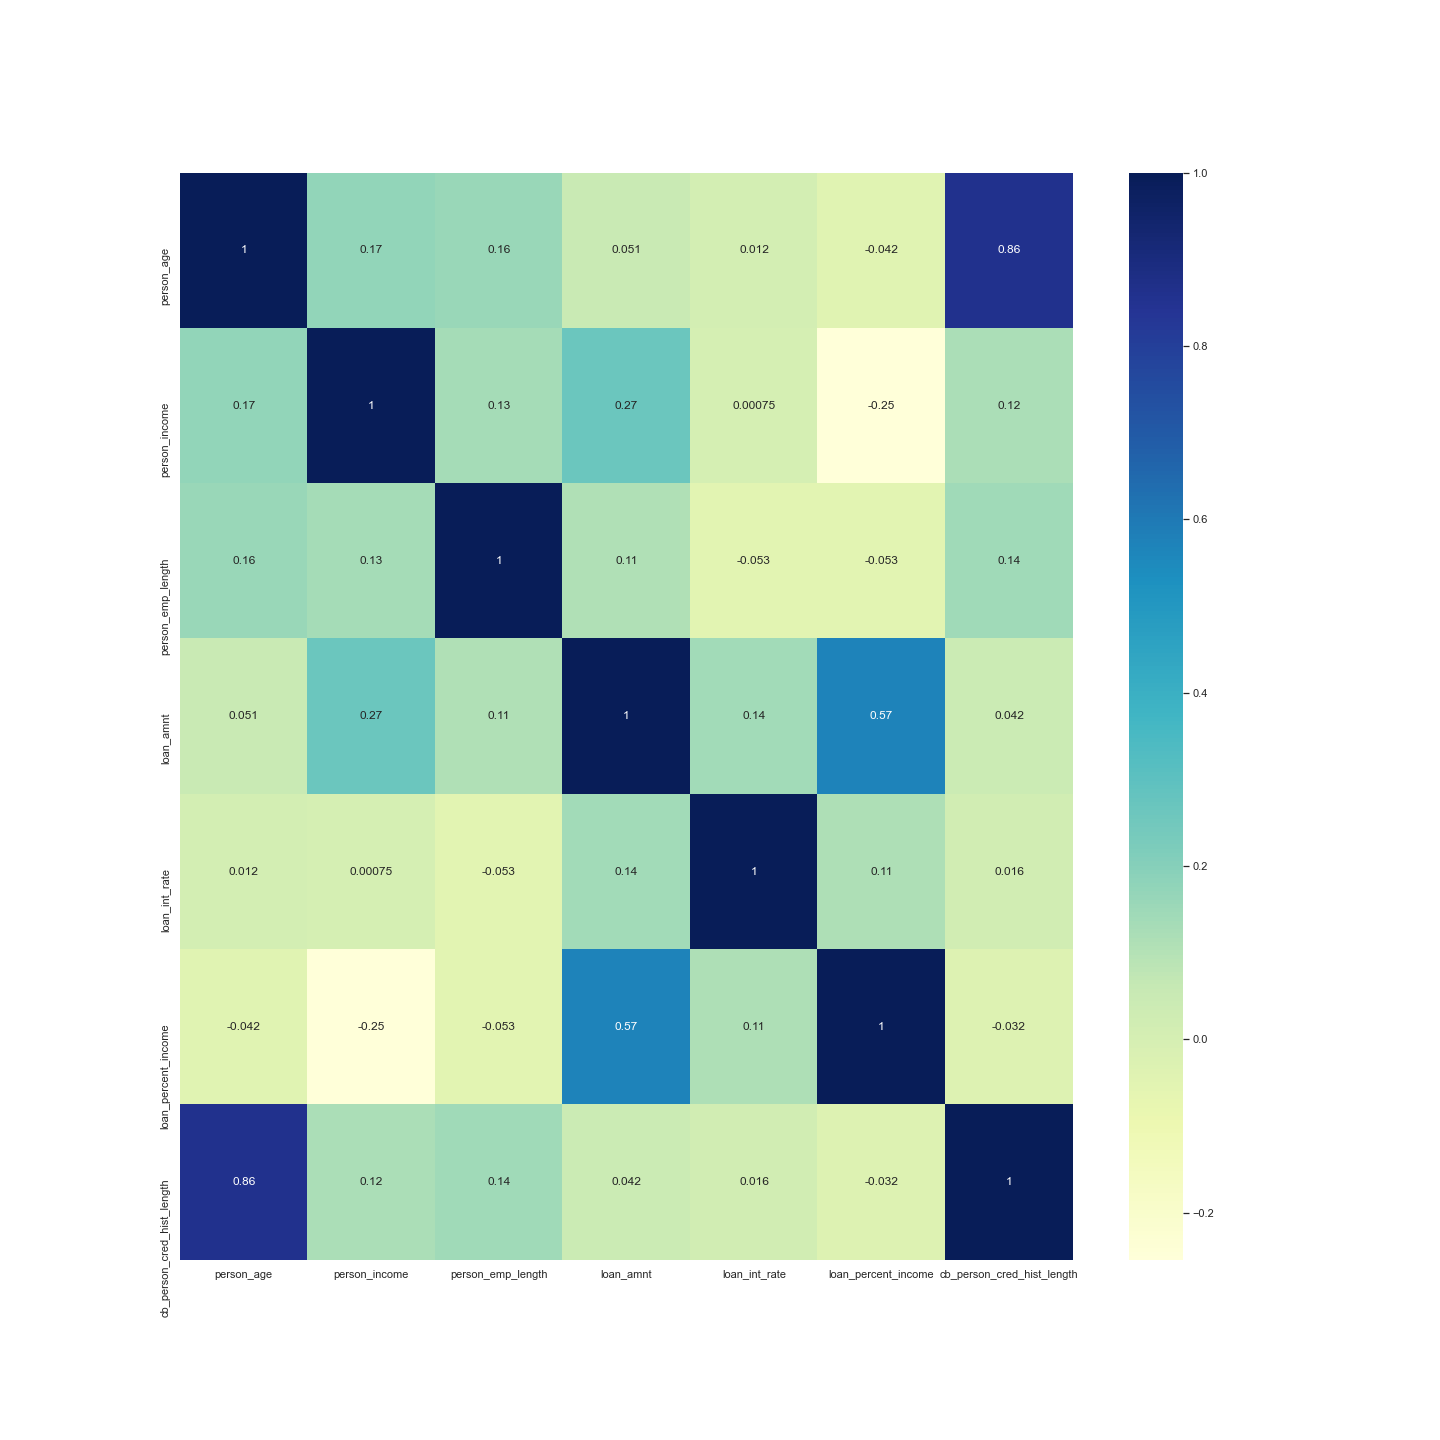
\includegraphics[width=10cm, height=8cm]{coorelation_heapmatap.png}
\caption{Co-relation Heat map}
\end{figure}

\begin{figure}[!htb] % h - Place the float here, i.e., approximately at the same point it occurs in the source text (however, not exactly at the spot)
\centering
\includegraphics[width=9cm, height=6cm]{pairplot.png}
\caption{Pair plot among numerical features}
\end{figure}




\subsubsection{Findings from EDA}


We made Treemap for Age-Person Income-Loan amount (Figure 6)
From the below Figure 6 we can observe, what is the loan amount that different age groups of people with different income ranges are requesting.
As you can observe from the above TreeMap shows the different ages when you go into those different ages groups it shows their Income and If we filter with different income's bracket we can see their requested loan amount for different Income bracket for that selected age group.
so from Figure 6 we can interpret that people with age 22-28 have more loan applications than others.
\begin{figure}[!h] % h - Place the float here, i.e., approximately at the same point it occurs in the source text (however, not exactly at the spot)
\centering
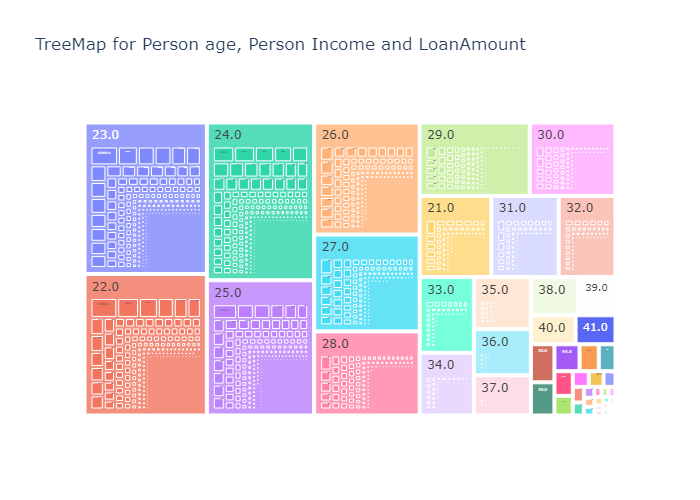
\includegraphics[width=10cm, height=8cm]{treemap1.png}
\caption{TreeMap for Person Age, Person Income and Loan Amount}
\end{figure}

We made a bar plot on the categorical variable person home ownership with the target variable loan status (Figure 7).From the plot we can notice that people who live in rented places are more likely to default when compared to others, who are least likely to default.
\begin{figure}[!h] % h - Place the float here, i.e., approximately at the same point it occurs in the source text (however, not exactly at the spot)
\centering
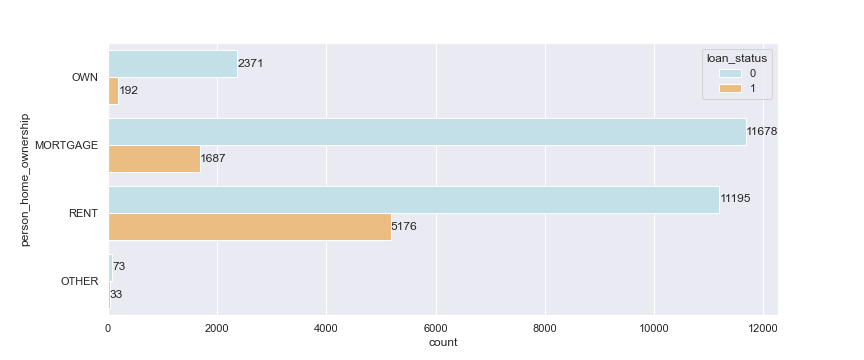
\includegraphics[width=10cm, height=8cm]{1_bar_plot_catagorical.png}
\caption{Bar plot for Person home ownership}
\end{figure}
 
 
 \begin{figure}[!h] % h - Place the float here, i.e., approximately at the same point it occurs in the source text (however, not exactly at the spot)
\centering
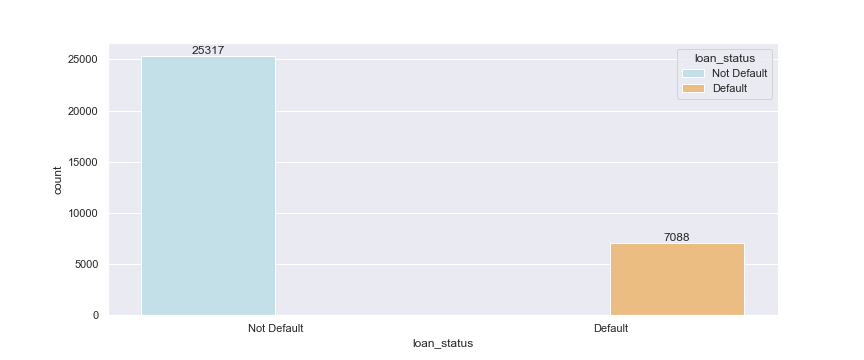
\includegraphics[width=10cm, height=8cm]{4_bar_plot_catagorical.png}
\caption{Bar plot for loan status}
\end{figure}
 From the Figure 8 , we can observe that the dataset is imbalanced as the cases where the frequency of loans being rejected are far less than the frequency of loans that are being approved. We can interpret that the dataset is biased towards 'not default'.As a result, we should use up sampling and try to balance the dataset.

\section{Model Training and Testing}

\subsection{Data Processing before training}
\subsubsection{One hot encoding}
Since we have a few categorical columns in the dataset which are ordinal and containing few categories, we can use one hot encoding on those features to make use of these features on models like Logistic Regression and XGBoost. We used OneHotEncoder() from the scikit-learn library on the dataset. From the below image we can see the one hot encoded data.
\begin{figure}[h] % h - Place the float here, i.e., approximately at the same point it occurs in the source text (however, not exactly at the spot)
\centering
\includegraphics[width=15cm, height=4cm]{OneHotEncodedData.png}
\caption{Dataset after One hot encoding}
\end{figure}

\subsubsection{Train Test split}
Train-Test split is a strategy for measuring the performance of a machine learning algorithm. As we are using supervised learning technique for classification or regression task train and test split would be helpful.
We have divided dataset into two subsets as part of the train-test. The training dataset is the initial subset, which is used to fit the model. The second subset is not used to train the model; instead, the dataset's input element is given to the model, which then makes predictions and compares them to the predicted values.

\subsubsection{Upsampling the Training data}
When working with unbalanced datasets, the problem is that most machine learning techniques approaches will overlook the minority class, resulting in poor performance, even though it is often the minority class that is most relevant. One of the approaches to address an imbalanced dataset is to oversample the minority class.
Upsampling is a procedure where the synthetically generated data points are introduced into the dataset. Following this procedure results in counts of both the labels being almost identical. This procedure prevents the model from overlooking the minority class and inclining towards the majority class.


\begin{figure}[!htb]
     \centering
     \begin{subfigure}[b]{0.3\textwidth}
         \centering
         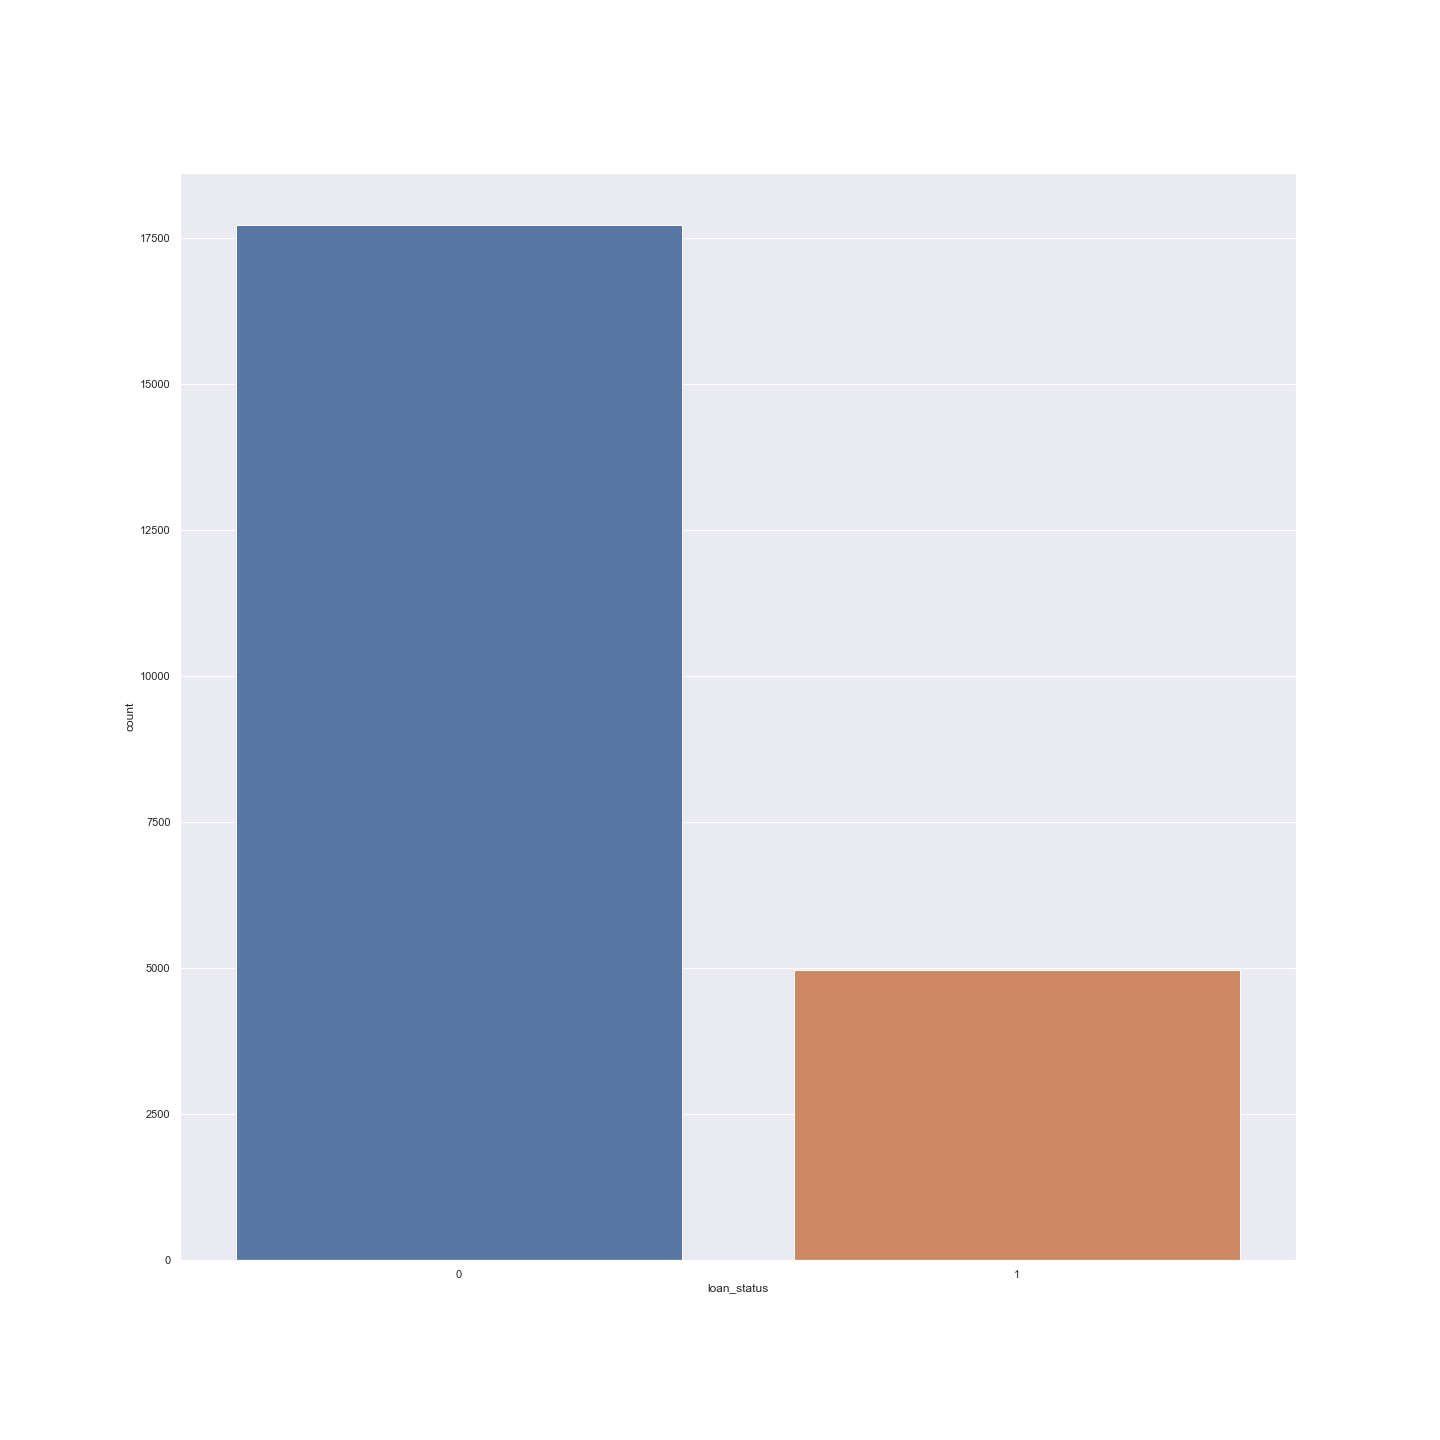
\includegraphics[width=6cm, height=8cm]{before_upsampling.png}
         \caption{Before Upsampling}
         \label{fig:RF}
     \end{subfigure}
     \hfill
     \begin{subfigure}[b]{0.3\textwidth}
         \centering
         \includegraphics[width=6cm, height=8cm]{after_upsampling.png}
         \caption{After Upsampling}
         \label{fig:DT}
     \end{subfigure}
     \hfill
     \caption{Countplot before and after Upsampling}
\end{figure}

After dividing the dataset into two subsets as training set and test set, we performed upsampling only on the training subset using SMOTE (Synthetic Minority Over-sampling Technique) from imblearn.


\subsection{Models Training and Parameter Tuning}

For solving the problem we have applied multiple models on the dataset.
Below are the few models we applied and the processes involved.
 
\subsubsection{Random Forest Classifier}

In this module, we will create several random forest models for our dataset and see which of them works best. We will create a simple random forest, then tune its parameters using GridSearchCV, and then form a model using only the features selected through the SelectFromModel() method. As our dataset is imbalanced, we first upsample it and then use it to train our models.

Initially, we create a simple random forest classifier, with max\_depth set to 3. Even though the f1 scores are good for both classes in the training dataset, the f1 score for class 1 isn't the best in the test dataset. As a next step, we will use the GridSearchCV() method to tune the hyper-parameters. In the random forest classifier, we set appropriate ranges for all parameters and tuned them to get the best results. The best\_params\_ variable is used to fetch the parameter values, which are then used to form a random forest classifier. The f1 score has increased significantly for class 1 in the test dataset as well as for both classes in the training and test datasets. There is slight overfitting in the dataset with 97\% for the training data and 93\% for the testing data. We will examine if we can reduce this overfitting by using only the top features needed for the model. We use the SelectFromModel() method to select our previous model. SelectFromModel() extracts the most significant features from the given data, based on their weights. Fit the train data into the SelectFromModel() with our model then use the get\_support() function to get the top features. These top\_features are then used to train the previously tuned model. We can see from the results that we did not achieve what we expected, but rather the f1 score of class 1 decreased. The overfitting was also not reduced. Out of these 3 models, the second, hyper-parameter-tuned model performs the best.

\subsubsection{Decision Tree Classifier}
As the decision tree's are widely used in banking sector, we have created Decision Tree model for our dataset. Decision Tress are easy to interpret. After a little explanation, we can grasp decision tree models, but decision-tree learners can produce too complicated trees that do not generalize data well. For this overfitting problem we tried to solve using techniques like pruning.
Results of the decision tree algorithm on the dataset are much more interesting than Logistic Regression as we got 89\% accuracy.

\subsubsection{Logistic Regression}
Logistic regression is one of the popular machine learning techniques which comes under the category of supervised learning techniques. It’s used for predicting categorically dependent variables using a set of independent variables. It is widely used for binary classification like yes or no , default or not default. Logistic Regression is relatively faster than other supervised classification techniques or ensemble methods, but it is less accurate. With logistic regression we got an accuracy of 81\% and precision of 55\%.

\subsubsection{XGBoost Classifier}
For solving this problem we implemented XGBoost agorithm.This algorithm uses Gradient boosting technique and trees to understand the data patterns. About model, it is an  ensemble method, meaning it’s a way of combining predictions from several models into one. It does that by taking each predictor sequentially and modelling it based on its predecessor’s error.

Because of its accuracy and simplicity, it has become one of the most used machine learning techniques. We can use this model for both regression and classification.

After applying up-sampling and encoding techniques,we have trained the model on the resulting dataset.The reason for considering this algorithm is that,we have converted the entire dataset to numerical,and tree based algorithms create the best splits on numerical data.Instead of creating complex equations making the model complicated these tree base models create simple yet powerful models.

We received 93\% accuracy on the test dataset,and AUC metric is 0.95 which tells us that model is able to differntiate classes very well. 

\section{Comparisions}

After applying multiple models on the dataset we have monitored results from each model. We compare these results and come to a conclusion on the best model suited to solve this problem.
The metrics we have used to find the generalized model are:

\begin{itemize}
  \item Accuracy
  \item Precision
  \item Re-Call
  \item F-1 Score
  \item ROC-AUC 
 \end{itemize}
 
Below are the evaluation metrics across all the models.

\begin{table}[!ht]
    \centering
    \begin{tabular}{|l|l|l|l|l|}
    \hline
        Model & Accuracy & Precision & Recall & F1-Score \\ \hline
        RandomForestClassifier & 0.900432 & 0.825745 & 0.690644 & 0.752176 \\ \hline
        DecisionTreeClassifier & 0.890249 & 0.73917 & 0.770099 & 0.754317 \\ \hline
        XGBClassifier & 0.933244 & 0.941986 & 0.74048 & 0.829166 \\ \hline
        LogisticRegression & 0.811767 & 0.550084 & 0.766808 & 0.640613 \\ \hline
    \end{tabular}
    \caption{Evaluation metrics across different models}
\end{table}


\begin{figure}[!htb]
     \centering
     \begin{subfigure}[b]{0.3\textwidth}
         \centering
         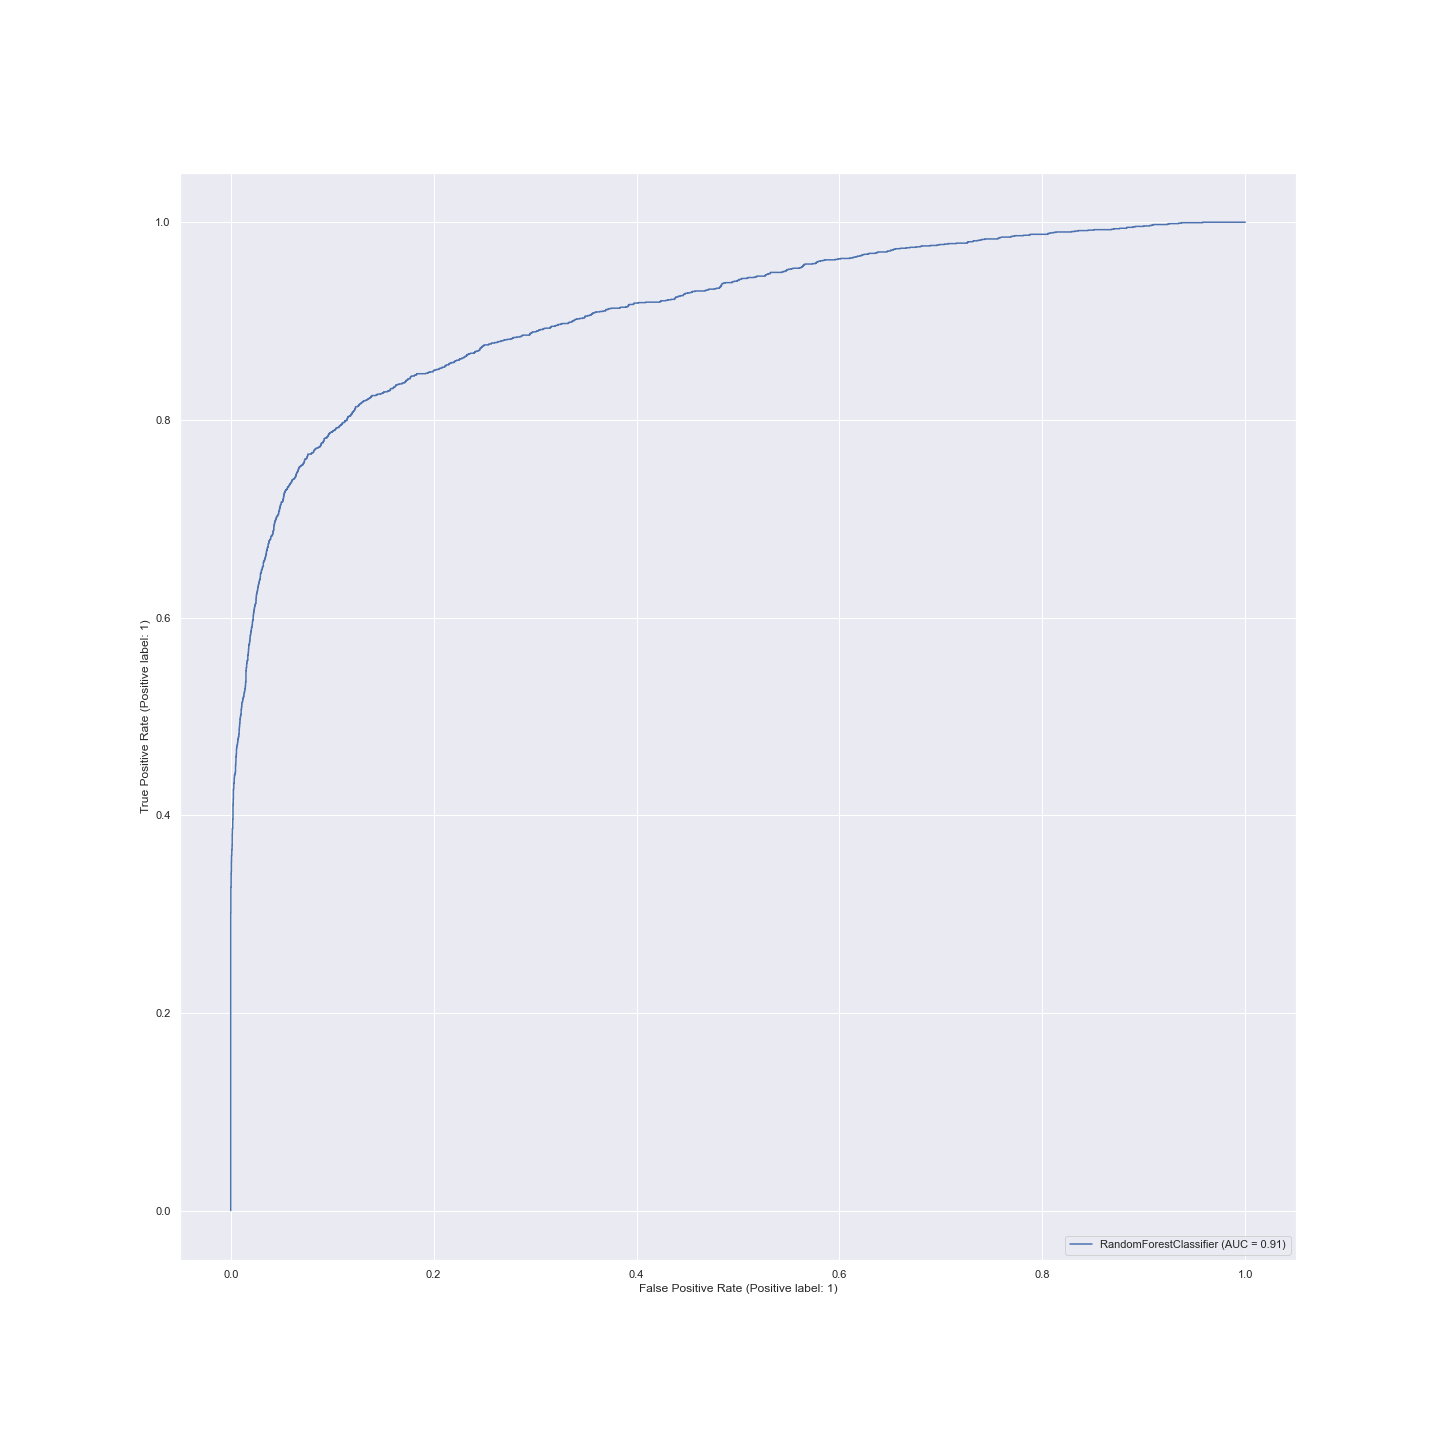
\includegraphics[width=8cm, height=8cm]{RandomForestClassifier_roc_auc_plot.png}
         \caption{Random Forest ROC-AUC(0.91)}
         \label{fig:RF}
     \end{subfigure}
     \hfill
     \begin{subfigure}[b]{0.3\textwidth}
         \centering
         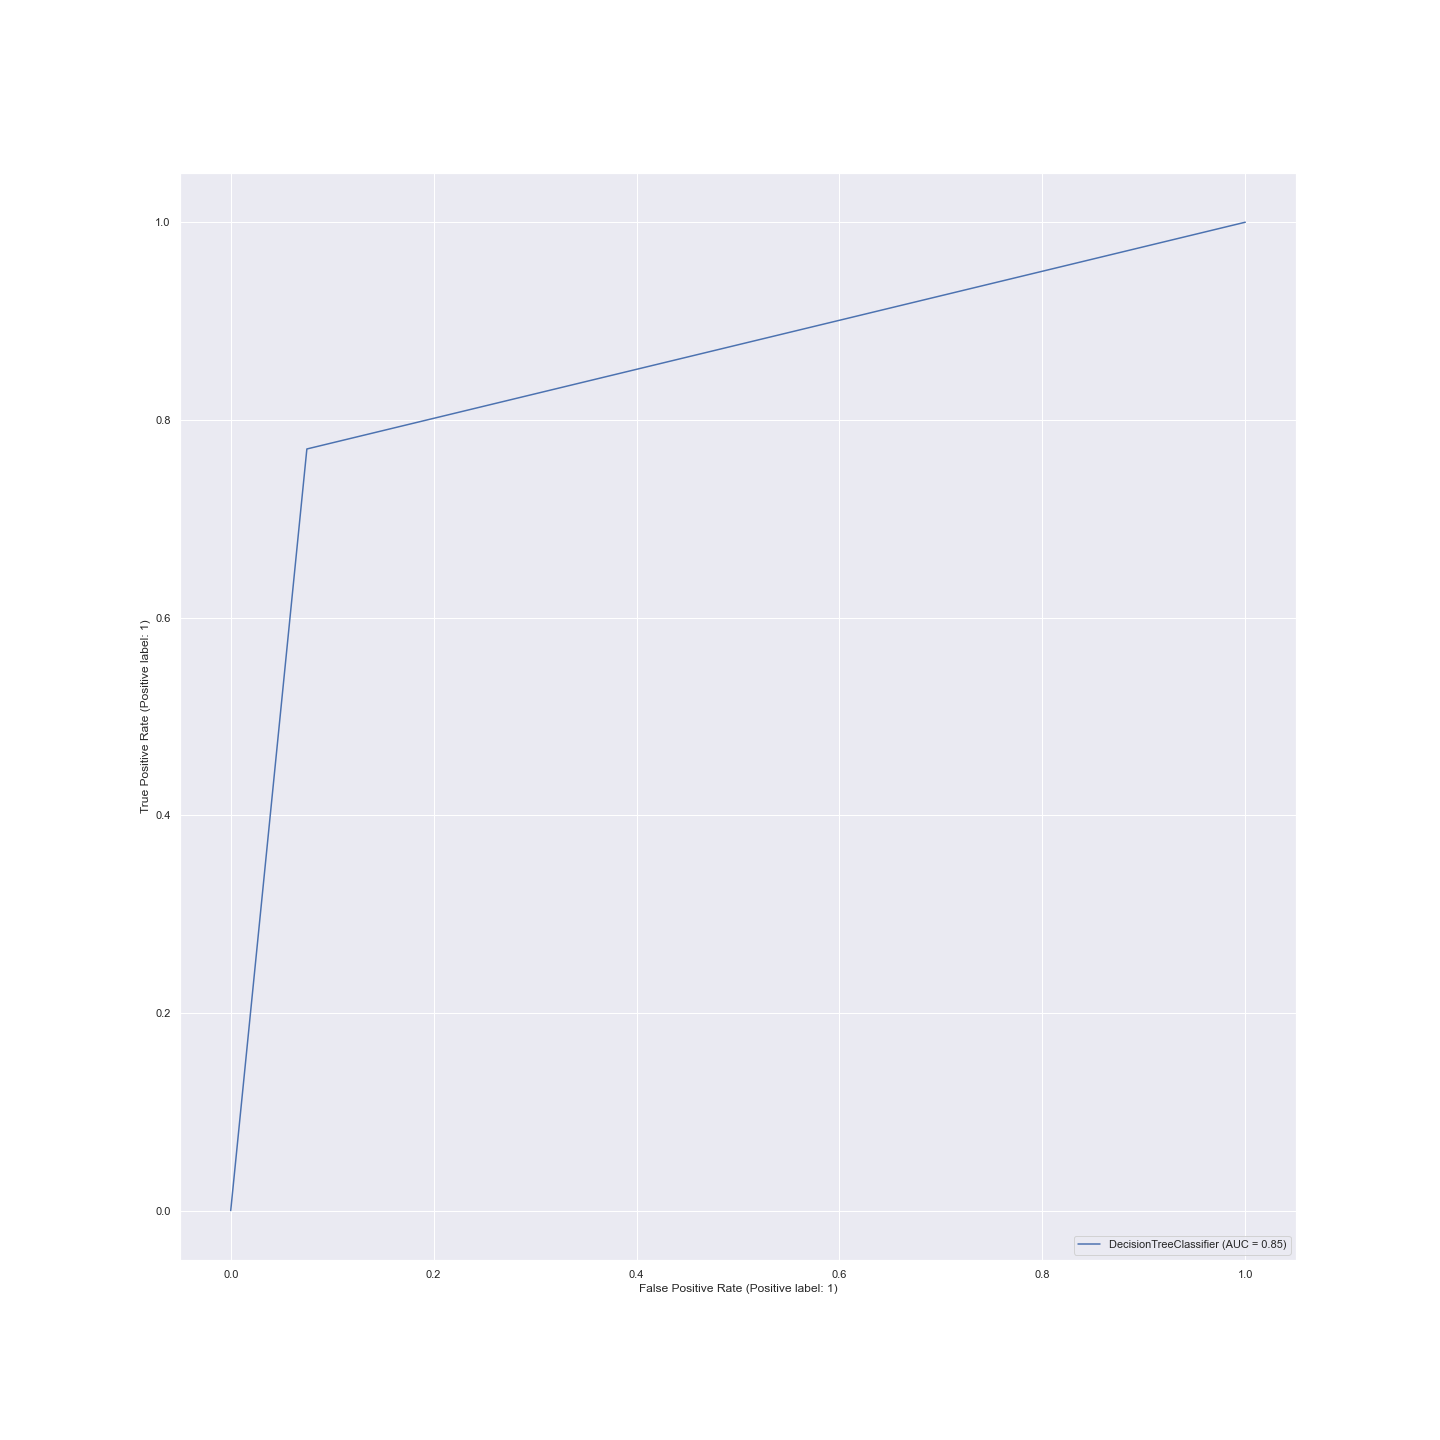
\includegraphics[width=8cm, height=8cm]{DecisionTreeClassifier_roc_auc_plot.png}
         \caption{DecisionTreeClassifier ROC-AUC(0.85)}
         \label{fig:DT}
     \end{subfigure}
     \hfill
        \caption{ROC AUC Curves for Random Forest and Decision Tree classifiers}
        \label{fig:ROC AUC}
\end{figure}

\begin{figure}[!htb]
     \centering
     \begin{subfigure}[b]{0.3\textwidth}
         \centering
         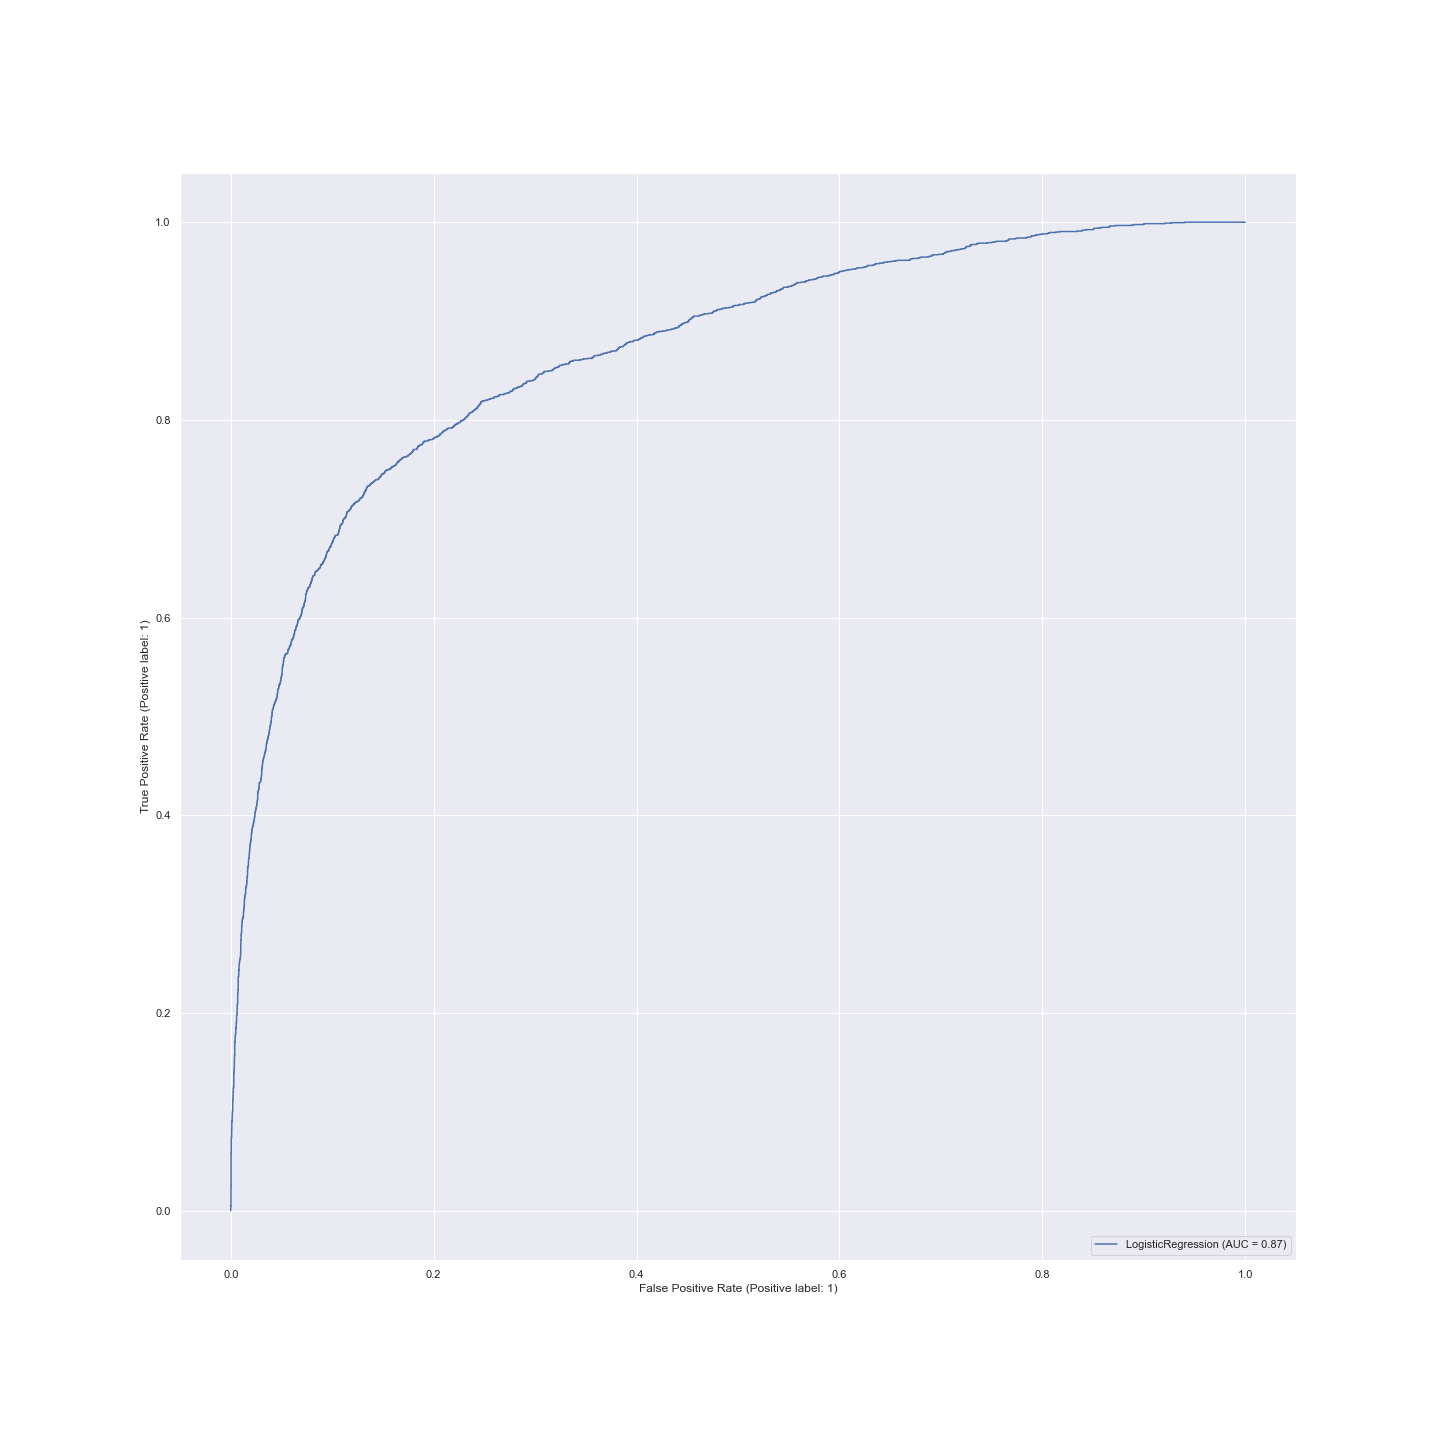
\includegraphics[width=8cm, height=8cm]{LogisticRegression_roc_auc_plot.png}
         \caption{LogisticRegression ROC-AUC(0.87)}
         \label{fig:DT}
     \end{subfigure}
     \hfill
     \begin{subfigure}[b]{0.3\textwidth}
         \centering
         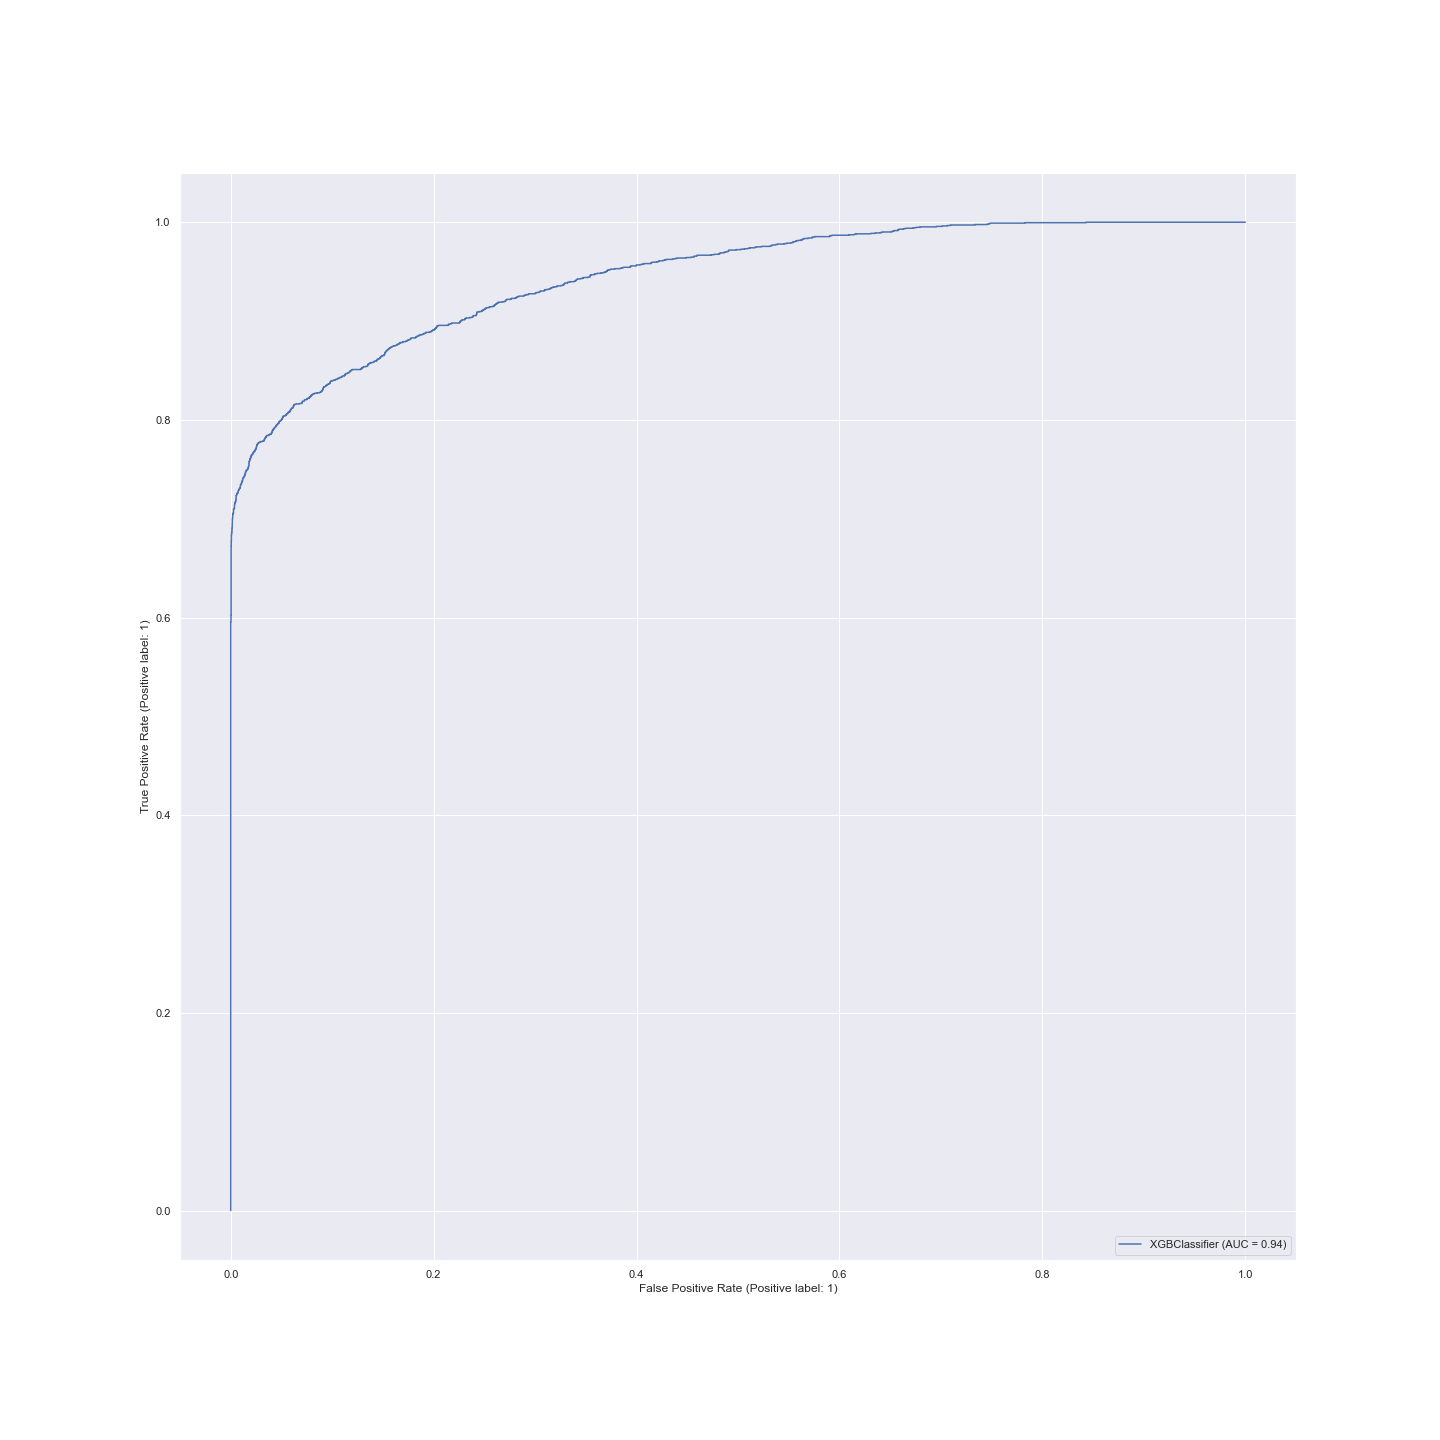
\includegraphics[width=8cm, height=8cm]{XGBClassifier_roc_auc_plot.png}
         \caption{XGBClassifier ROC-AUC(0.94)}
         \label{fig:XGB}
     \end{subfigure}
        \caption{ROC AUC Curves for LogisticRegression and XGBoost classifiers}
        \label{fig:ROC AUC}
\end{figure}

Out of all the models tested and evaluated, XGBoost and Random Forest delivered high performance in identifying the classes Default and Not Default.



\pagebreak
\section{Conclusion}
After evaluating the performance of all the models,we understand that tree based models are best suited for this dataset.Bagging models like Random Forest and Boosting models like XGBoost delivered similar results.

Though the dataset is balanced by duplicating the minority class,adding additional data points in future might make the model much robust.To add strength to the model,in future we plan to add additional features to the dataset and testing it with neural networks.

% \section{}
\begin{thebibliography}{}


\bibitem{}
Farzad, Shahbazi (2019), \emph{ Using decision tree classification algorithm to design and construct the credit rating model for banking customers.}

\bibitem{research paper}
Tzu-Tsung Wong, Shang-Jung Yeh(2019), \emph{Weighted Random Forests for Evaluating Financial Credit Risk}
\bibitem{research paper}
Ali Al-Aradi(2014), \emph{Credit Scoring via Logistic Regression}
\bibitem{research Paper}
Oliver Takawira, John W.Muteba Mwamba (2022), \emph{Sovereign Credit Ratings Analysis Using the Logistic Regression Model}
\bibitem{research paper}
Kui Wanga, Meixuan Li, Jingyi Cheng, Xiaomeng Zhou, Gang Li (2022), \emph{Research on personal credit risk evaluation based on XGBoost}

\end{thebibliography}
\end{document}
